\section{Durchführung}
\label{sec:Durchführung}

Im ersten Teil des Versuchs wird die Proportionalität zwischen der Ablenkspannung und der
Verschiebung des Auftrefforts des Elektrons untersucht. Hierzu werden fünf unterschiedliche
Beschleunigungsspannungen verwendet, die so reguliert werden, dass der Auftreffort auf den
neun äquidistanten Linien auf dem Detektorschirm liegt. Die zugehörigen Spannungen werden notiert.
Die verwendete Schaltung ist in Abbildung 4 dargestellt.
\begin{figure}[H]
  \centering
  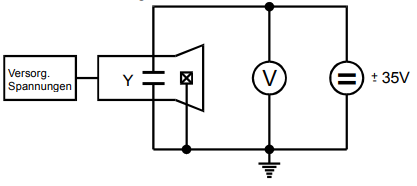
\includegraphics[height=4cm]{schalt1.png}
  \caption{Schaltung zur Untersuchung der Proportionalität zwischen Ablenkspannung und Verschiebung des Auftreffortes. \cite[S.5]{kent}}
\end{figure}

Im zweiten Teil wird ein Kathodenstrahloszillograph nach Abbildung 5 konstruiert. Hierbei wird
die Sägezahnfrequenz so eingestellt, dass auf dem Oszillographen stehende Bilder der angelegten
Sinusspannung zu sehen sind. Die Fälle $n = \frac{1}{2}, 1, 2, 3$ werden realisiert und die
zugehörige Sägezahnfrequenz wird notiert.

\begin{figure}[H]
  \centering
  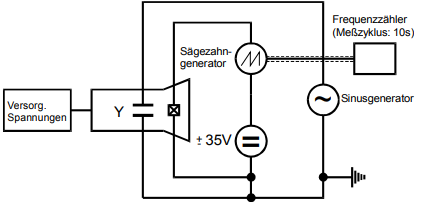
\includegraphics[height=4cm]{schalt2.png}
  \caption{Schaltung zum Bau eines Kathodenstrahloszillographen. \cite[S.5]{kent}}
\end{figure}

Im dritten Teil wird die spezifische Elektronenladung mittels der Ablenkung des Elektronenstrahls
durch das homogene Magnetfeld einer Helmholtzspule bestimmt. Die Kathodenstrahlröhre wird zunächst mithilfe
eines speziellen Kompass (Deklinatorium/Inklinatorium) in Nord-Süd-Richtung gedreht um den Einfluss
des Erdmagnetfelds so gering wie möglich zu halten. Es wird für zwei verschiedene konstante
Beschleunigungsspannungen die Strahlverschiebung in Abhängigkeit des Magnetfelds notiert, indem dieses
so reguliert wird, dass die Elektronen auf die neun äquidistanten Linien des Detektorschirms treffen.

Zuletzt wird die Intensität des Magnetfeldes am Versuchsort ermittelt. 
Hierzu bestimmt man zunächst den Inklinationswinkel, also den Winkel zwischen Horizontalebene
und der Richung des Erdfeldes, indem man das Inklinatorium aus voriger Position um 90° schwenkt,
sodass die Drehachse der Nadel horizontal liegt. Der Winkel wird abgelesen.
Anschließend wird die Position des Auftreffortes der Elektronen bei ausgeschalteter Helmholtzspule
und möglichst niedriger Beschleunigungsspannung vermerkt. Die Versuchsanordnung wird in Ost-West-Richtung ausgerichtet,
sodass das Magnetfeld der Erde den Elektronenstrahl ablenkt. Der Strom der Helmholtzspule wird
so reguliert, dass das erzeugte Magnetfeld dem der Erde entgegenwirkt und die Elektronen
am ursprünglichen Ort auf den Detektorschirm treffen. Der hierzu benötigte Strom wird notiert.
